\documentclass[conference]{IEEEtran}
\IEEEoverridecommandlockouts
% The preceding line is only needed to identify funding in the first footnote. If that is unneeded, please comment it out.
%Template version as of 6/27/2024

\usepackage{cite}
\usepackage{amsmath,amssymb,amsfonts}
\usepackage{algorithmic}
\usepackage{graphicx}
\usepackage{textcomp}
\usepackage{booktabs}
\usepackage{multirow}
\usepackage{fancyhdr}
\usepackage[hidelinks]{hyperref}
\usepackage{lipsum}
\usepackage{xcolor}

\def\BibTeX{{\rm B\kern-.05em{\sc i\kern-.025em b}\kern-.08em
    T\kern-.1667em\lower.7ex\hbox{E}\kern-.125emX}}
\renewcommand{\IEEEkeywordsname}{Keywords}

% Custom header & footer
\pagestyle{fancy}
\chead{SISPAD 2026, September 28-30, 2026, Kumamoto, Japan}
\cfoot{SISPAD 2026 - https://sispad2026.jp/}
\let\oldheadrule\headrule% Copy \headrule into \oldheadrule
\renewcommand{\headrule}{\oldheadrule}
\let\oldfootrule\footrule% Copy \footrule into \oldfootrule
\renewcommand{\footrule}{\oldfootrule}
\renewcommand{\footrulewidth}{0.1pt}

\begin{document}

\title{PhysAgent: Physics-Informed SDevice Code Generation via Ontology-Guided LLM\\
}

% 저자 정보를 정의하는 부분
\author{
\begin{tabular}{c@{\hspace{1.6cm}}c}
Shinbin Kim$^{*}$ & Giung Kim$^{*}$ \\
\textit{Semiconductor Engineering Department} & \textit{Semiconductor Engineering Department} \\
\textit{POSTECH} & \textit{POSTECH} \\
Pohang, Republic of Korea & Pohang, Republic of Korea \\
\href{mailto:sinbin0701@postech.ac.kr}{sinbin0701@postech.ac.kr} & \href{mailto:giung0408@postech.ac.kr}{giung0408@postech.ac.kr}
\end{tabular}
\thanks{$^{*}$These authors contributed equally to this work.}
}

\maketitle
\thispagestyle{fancy}

\begin{abstract}
As the limits of semiconductor scaling become increasingly evident, the importance of DTCO and TCAD continues to grow. However, the core challenge of TCAD lies not in simple structure generation, but in configuring Sdevice physics and generating parameter files, which require deep understanding of physical models and domain-specific knowledge. To address this challenge, we propose PhysAgent. Instead of relying on synthetic training data, PhysAgent builds a Sentaurus TCAD guide-based ontology that structures physical models, equations, conditions, parameters, and their relationships, and further integrates literature-driven domain knowledge to generate physically grounded Sdevice files. In this way, PhysAgent goes beyond template-level code generation and demonstrates the potential to support expert-level modeling workflows for specific semiconductor materials.

\end{abstract}

\begin{IEEEkeywords}
TCAD, ontology, physics-informed modeling, parameter file generation, domain knowledge, semiconductor materials
\end{IEEEkeywords}

\section{Introduction}
This document is a proposed template and guideline for SISPAD 2026. It is based on IEEE template example. For more details, please refer to the IEEE template example available at https://www.ieee.org/conferences/publishing/templates.html .


\section{Related Work}
TCAD simulation consists of SDE for device geometry and SDevice for physics models and solver settings. While LLMs have been applied to SDE code generation through fine-tuning or in-context learning, SDevice configuration---selecting and parameterizing models such as mobility, recombination, and bandgap narrowing---remains unaddressed due to its high expertise requirements.


\section{Proposed Framework}
PhysAgent combines a TCAD physics ontology and literature-driven domain knowledge to guide LLM-based SDevice file generation. The constructed ontology is publicly available as an interactive web platform~\cite{ontology_tcad}.

\subsection{TCAD Physics Ontology}
An SDevice simulation takes a command file (\texttt{.cmd}) and a parameter file (\texttt{.par}) as input. The physics block in the \texttt{.cmd} file specifies the physical models activated for each material, while the \texttt{.par} file defines the parameters required by these models along with fundamental properties such as bandgap, permittivity, and the DOS effective masses of electrons and holes. Thus, the model selection in the \texttt{.cmd} file determines the parameter set that must be provided in the \texttt{.par} file.
To consistently capture this \texttt{.cmd}--\texttt{.par} dependency, we structure the relevant parameters, TCAD syntax, and physical knowledge into an ontology grounded in {\color{red}the Poisson and transport equations, together with the governing equations of each physical model}. {\color{red}Each parameter and each physical-model equation is represented as a node. Parameter nodes attach to the equation node of the model they belong to (membership), and equation nodes link to one another to capture inter-model couplings (coupling). Given a model selection, traversing these edges yields the required parameter set.} A syntax layer then applies the SDevice syntax to the selected equations and nodes to generate the \texttt{.cmd} and \texttt{.par} files (Fig.~\ref{fig:ontology}).

\subsection{Ontology-Guided Generation}
Given a target device and material, PhysAgent accesses the ontology through an MCP (Model Context Protocol) interface {\color{red}(referred to as \texttt{ontology\_mcp})} that exposes four tools. \texttt{ontology\_overview} returns the node/edge map of the graph, serving as the entry point for grasping the overall structure. \texttt{ontology\_get\_chapter} identifies the governing equations associated with a selected node and derives the parameter set required by those equations. \texttt{ontology\_get\_syntax} provides the SDevice syntax template for each model, specifying keyword names, section layout, and required fields. \texttt{ontology\_get\_reference} returns material-specific parameter values together with per-parameter source citations drawn from a curated collection of papers, datasheets, and TCAD references{\color{red}~\cite{bludau1974, ioffe_nsm}}. In our experiments, we employ Claude Sonnet, whose context window is limited to 200k tokens, whereas the full ontology measures $\sim$458k tokens and therefore cannot be injected directly into the prompt. The MCP-based selective retrieval scheme circumvents this limitation by allowing the LLM to query only the information required at each step, keeping the per-query context well within the 200k-token budget. Moreover, each parameter in the generated \texttt{.par} inherits the citation returned by \texttt{ontology\_get\_reference}, thereby enabling parameter-level provenance (Fig.~\ref{fig:exp2}).



\section{Result}
PhysAgent targets the physics specification stage---the SDevice \texttt{Physics} block and \texttt{.par} file---while structure (\texttt{.tdr}), solver, and bias schedule remain fixed, orthogonal to prior structure-generation work~\cite{nguyen, malts}. Three generators share the same base LLM and prompt: \textit{Vanilla} (spec only), \textit{LLM+Guide} (spec + Sentaurus manual), and \textit{PhysAgent} (spec + ontology + literature). We validate three claims.

\textbf{Successful TCAD Execution.}
On a Si nMOSFET we compare three modes (Vanilla, LLM+Guide, PhysAgent) across three prompt levels (L1--L3: explicit model list, categories, intent only), three trials each. Vanilla and LLM+Guide produce characteristic syntactic errors---invented model names, undefined parameters, malformed material blocks---lacking any structural anchor, whereas PhysAgent copies directly from typed ontology nodes at {\color{red}48$\times$} smaller prefill than LLM+Guide. Across L1$\to$L3 model coverage tracks prompt specificity: which physical mechanisms the deck selects depends on what the prompt asserts, making phenomenon-level prompting central to the simulation's analytical scope ({\color{red}Fig.~\ref{fig:exp1}}).

\textbf{Literature-Grounded Parameter File Generation.}

\textbf{Phenomenon-Driven Model Selection and Deck Construction.}


\begin{figure}[htbp]
    \centerline{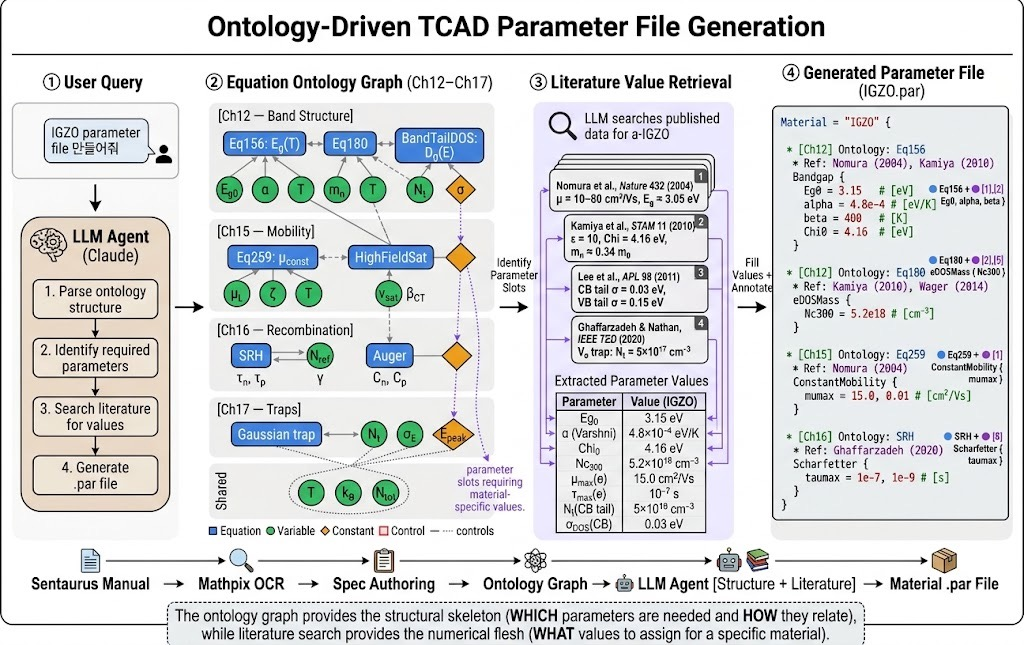
\includegraphics[width=\columnwidth]{Fig/framework.jpg}}
    \caption{PhysAgent framework overview.}
    \label{fig:all}
\end{figure}

\begin{figure}[htbp]
    \centerline{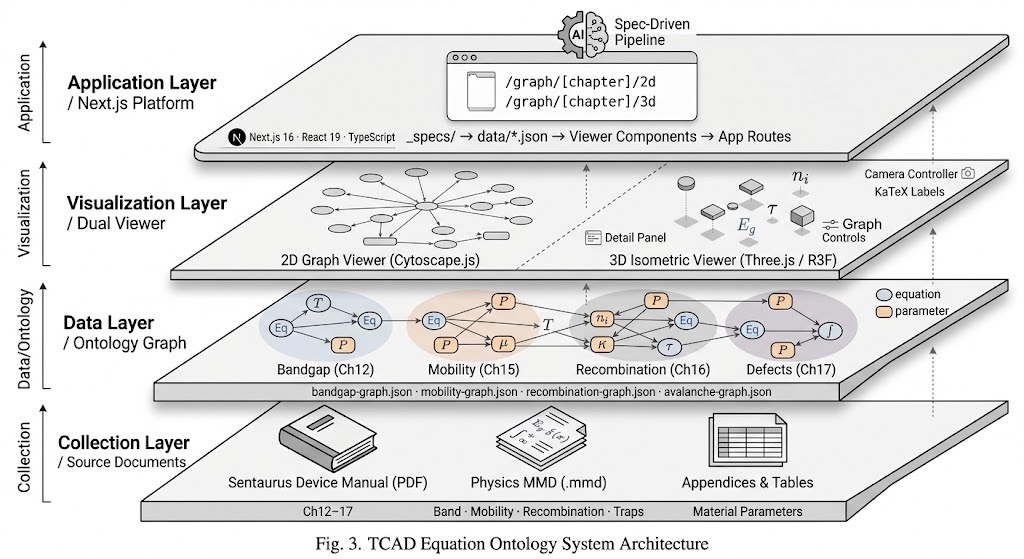
\includegraphics[width=0.8\columnwidth]{Fig/ontology.jpg}}
    \caption{Ontology system architecture.}
    \label{fig:ontology}
\end{figure}

\begin{figure}[htbp]
    \centerline{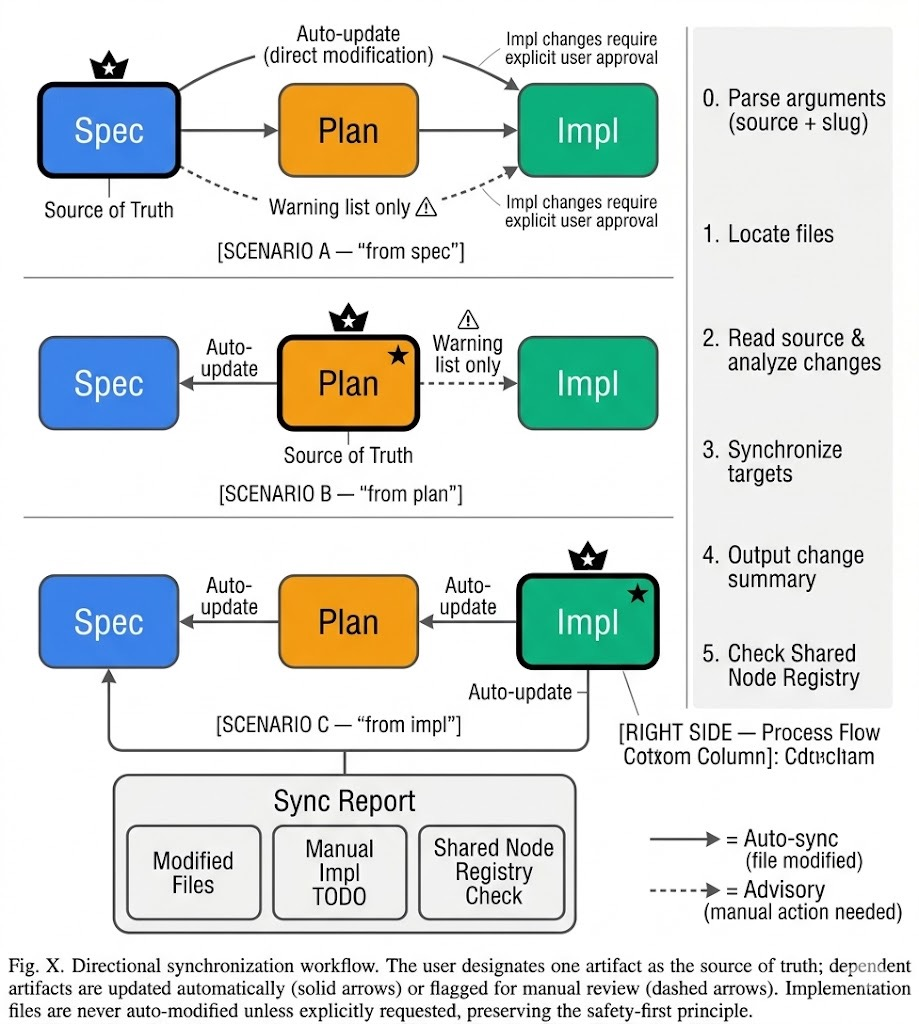
\includegraphics[width=0.8\columnwidth]{Fig/expansion.validation_model.jpg}}
    \caption{Expansion and validation workflow.}
    \label{fig:expansion}
\end{figure}

\section{Conclusion}
We presented PhysAgent, which generates physically grounded SDevice files by combining a TCAD guide-based ontology with literature-driven domain knowledge. Instead of relying on scarce synthetic training data, PhysAgent builds explicit knowledge structures that enable general-purpose LLMs to support expert-level TCAD modeling workflows.


\begin{thebibliography}{00}
\bibitem{dtco} Z. Ji \textit{et al.}, ``Toward reliability- and variability-aware design-technology co-optimization at advanced nodes,'' \textit{IEEE Trans. Electron Devices}, vol.~71, no.~1, pp.~138--150, 2024.
\bibitem{synopsys_tcad} Synopsys, ``Sentaurus TCAD,'' 2025. [Online]. Available: https://www.synopsys.com/manufacturing/tcad.html
\bibitem{nguyen} L.~M.~L. Nguyen, A.~Lu, and H.~Y.~Wong, ``TCAD structure input file generation using large language model,'' in \textit{Proc. SISPAD}, 2024, pp.~1--4.
\bibitem{chattcad} Z.~Zhang, S.~Nassif, and M.~Tahoori, ``ChatTCAD: Leveraging large language models for automated TCAD simulation file generation,'' in \textit{Proc. ISVLSI}, 2025, pp.~1--6.
\bibitem{malts} J.~Dou \textit{et al.}, ``MALTS: A multi-agent large language model-based layout-to-TCAD structure synthesizer,'' in \textit{Proc. ISEDA}, 2025, pp.~795--800.
\bibitem{agentictcad} G.~Fan \textit{et al.}, ``AgenticTCAD: A LLM-based multi-agent framework for automated TCAD code generation and device optimization,'' \textit{arXiv:2512.23742}, 2026.
\end{thebibliography}

\end{document}
